% !TeX spellcheck = en_US
% !TeX encoding = UTF-8
% !TeX root = ../report.tex

\chapter{Implementation}
\label{chp:Implementation}

%write about implementation of ROS


\section{V-Disparity Implementation}
\label{vdisp_impl}


\section{Hardware}

%write more about settings and performance of zed camera, and lidar

The Gokart is fitted with a ZED Stereolabs camera, see Figure \ref{fig:zedproductmain}, which was the basis for the V-Disparity method. The camera comes with a ZED SDK, which provides many functionalities, such as disparity map generation and point cloud computation. The Python API enables quick and intuitive access to these functionalities.
In addition, a Velodyne VLD-16 Lidar is mounted on top of the Gokart, which can be seen in Figure \ref{fig:lidar}. It offers 16 scanning lines with high accuracy.
More infos on the used hardware can be found on the manufacturer's website.

\begin{figure}
	\centering
	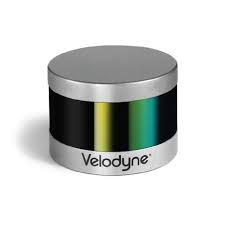
\includegraphics[width=0.5\linewidth]{Figures/lidar}
	\caption[Velodyne Vld-16 Lidar Sensor]{}
	\label{fig:lidar}
\end{figure}

\begin{figure}
	\centering
	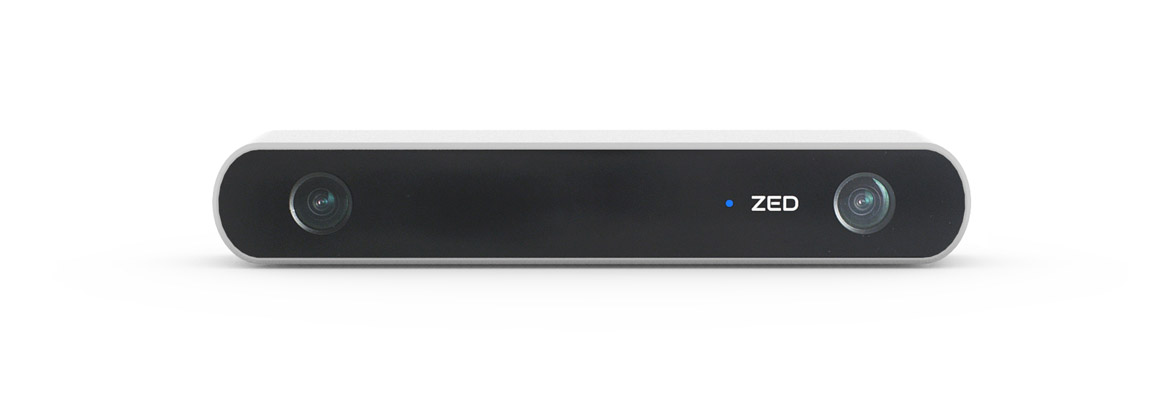
\includegraphics[width=0.7\linewidth]{Figures/ZED_product_main}
	\caption[ZED Stereolabs Camera]{}
	\label{fig:zedproductmain}
\end{figure}



\section{Code implementation}
\subsection{V-Disparity}

The method was implemented in the Python framework, while making use of the popular OpenCV library. OpenCV was used, mainly because of the existing methods already implemented, such as the probabilistic houghline transform, which was used for line-fitting. The OpenCV aims at real-time computer vision programming functions, which is a crucial property for autonomous vehicles.
\newline

Given the ZED Camera and the ZED SDK, data can be streamed from the Camera with few lines of code. Depending on the application, the resolution, framerate and other parameters can be adjusted accordingly. For disparity computation, range and quality can be modified, to fit the requirements.
The disparity map is computed as float32. For visualisation purposes, a normalisation and conversion to uint8 type needs to be done. 
For higher precision, the float32 disparity map can be used for further processing. 
To ease up on computation, the uint8 disparity map was used for the V-Disparity method. The number of histogram bins for every row histogram is then set to 255, one for every disparity value present in the normalised disparity image. OpenCV's calcHist function was used.
To extract the regions of interest, in our case the ground, OpenCV's Houghline transform can be used, to fit the line in the image. In order to fine tune the line fitting, probabilistic houghline transform was used, where minimum line length and maximum line gap can be adjusted. This line can then be backprojected into the original camera image, to generate the mask.

For the current implementation, the disparity map and camera images are streamed at a resolution of (672, 376). The same resolution is used for the V-Disparity Histogram and Line Fitting. For mask generation, the resolution was downscaled by a factor of two, to ease up on computation and enable real-time application. Using higher resolution could improve results, but drastically lowers the framerate

%insert figure of pipeline, from stereo image to disparity image to v-disparity image and fitted line, and finally the resulting mask.


In order to avoid speckles and disjointed mask segments, all mask pixels are labeled according to their connectedness, using OpenCV's connectedComponents function. Only the largest connected region is kept, all other labels are discarded. 

\subsection{Lidar to camera projection}
%write about how to construct rotation matrix

Euler angles where used to determine the rotation matrices. After constructing the rotation vector and determining the relative angles, the vector was transformed to a 3x3 rotation matrix. Because OpenCV only uses Rodrigues Vector notation for rotation, the rotation matrix had to be converted to Rodrigues as well. This was easily done with an already implemented OpenCV function.
There are two rotation and translation matrices which are used. The translation and rotation from the kart's center point to the camera is fixed and needs to be measured. The translation and rotation from the world coordinate origin to the kart's center points can be extracted from the generated odometry parameters.